%% slides.tex
%% Beamer presentation: Spacecraft CA SDec-POMDP
%% Compile: pdflatex slides.tex

\documentclass[aspectratio=169]{beamer}
\usetheme{Madrid}
\usecolortheme{seahorse}
\usepackage{amsmath, amssymb}
\usepackage{booktabs}
\usepackage{xcolor}
\usepackage{graphicx}

\definecolor{todo}{RGB}{200,50,50}
\newcommand{\TODO}[1]{\textcolor{todo}{\textit{[TODO: #1]}}}
\newcommand{\good}[1]{\textcolor{green!60!black}{#1}}
\newcommand{\bad}[1]{\textcolor{red!70!black}{#1}}

\title[Spacecraft CA SDec-POMDP]{Semi-Decentralized Multi-Spacecraft\\
Collision Avoidance under Communication Constraints}
\author{Grace Ra Kim, Mahdi Al-Husseini, Duncan Eddy, Mykel J.\ Kochenderfer}
\institute{Stanford University}
\date{\today}

% =============================================================================
\begin{document}
% =============================================================================

\begin{frame}
  \titlepage
\end{frame}

\begin{frame}{Outline}
  \tableofcontents
\end{frame}

% =============================================================================
\section{Motivation}
% =============================================================================

\begin{frame}{The Problem}
  \begin{columns}
    \begin{column}{0.55\textwidth}
      \textbf{LEO is getting crowded}
      \begin{itemize}
        \item Thousands of active satellites today
        \item SpaceX orbital data center: up to 1M satellites proposed
        \item More conjunctions, more CA decisions needed
      \end{itemize}
      \vspace{1em}
      \textbf{Current CA operations}
      \begin{itemize}
        \item Ground-driven, operator-specific
        \item Each operator gets CDMs, plans independently
        \item Limited by their own ground contact schedule
      \end{itemize}
    \end{column}
    \begin{column}{0.4\textwidth}
      \begin{block}{The Gap}
        \begin{itemize}
          \item Fully centralized: assumes perfect info
          \item Fully decentralized: ignores interaction
          \item \textbf{Neither models intermittent communication directly}
        \end{itemize}
      \end{block}
    \end{column}
  \end{columns}
\end{frame}

\begin{frame}{Our Approach}
  \begin{center}
    \large
    Model spacecraft CA as a\\[0.5em]
    \textbf{Semi-Decentralized POMDP (SDec-POMDP)}\\[0.5em]
    solved with \textbf{RS-SDA*}
  \end{center}
  \vspace{1em}
  \begin{itemize}
    \item Ground-station contact windows $=$ synchronization triggers
    \item Agents share beliefs \& coordinate \emph{only} during contacts
    \item \textbf{Asymmetric observations}: each agent observes miss distance
          based only on \emph{its own} maneuvers --- SC1 does not know SC2 burned
    \item Bridges centralized (always sync) and decentralized (never sync)
    \item Three scenarios quantify how communication structure shapes safety
  \end{itemize}
\end{frame}

% =============================================================================
\section{POMDP Formulation}
% =============================================================================

\begin{frame}{State Space}
  \begin{columns}
    \begin{column}{0.42\textwidth}
      \begin{block}{$s = (d_\text{miss},\; k)$}
        $d_\text{miss}$ = predicted miss at TCA (discretized)\\
        $k$ = planning stage (ground contact index)
      \end{block}
      \vspace{0.4em}
      \begin{tabular}{clc}
        \toprule
        Bin & Range & Risk \\
        \midrule
        0 & $[0, 1)$\,km   & \bad{Collision} \\
        1 & $[1, 5)$\,km   & \bad{High} \\
        2 & $[5, 20)$\,km  & Moderate \\
        3 & $[20, 100)$\,km & Low \\
        4 & $[100, 500)$\,km & Nominal \\
        5 & $[500+)$\,km   & \good{Safe} \\
        \bottomrule
      \end{tabular}\\[0.3em]
      \small 37 states total (6 bins $\times$ 6 stages + sink)
    \end{column}
    \begin{column}{0.55\textwidth}
      \textbf{Why miss distance?}
      \begin{itemize}
        \item What CDMs report; directly tied to reward
        \item Collapses 6D relative state to 1 scalar
        \item No comms variables needed --- sync is via contact-window triggers
      \end{itemize}
      \vspace{0.5em}
      \begin{alertblock}{WAIT $\Rightarrow$ same bin (key invariant)}
        Under no maneuver, predicted miss at TCA is unchanged --- Keplerian dynamics are deterministic. Starting in bin~0 means a collision \emph{will} happen unless a burn is applied before TCA.
      \end{alertblock}
    \end{column}
  \end{columns}
\end{frame}

\begin{frame}{Planning Horizon \& Rollout Timeline}
  \begin{columns}
    \begin{column}{0.48\textwidth}
      \begin{block}{``Init bin 0 at stage 0''}
        At $T{-}23.4$\,h, predicted miss $< 1$\,km.\\
        If nobody burns $\Rightarrow$ collision at TCA.\\[0.3em]
        \emph{When and how should each operator burn, given only noisy GS updates?}
      \end{block}
      \vspace{0.5em}
      \textbf{Contact windows from Brahe}\\
      \small Goddard GS (39°N, 77°W), 10° min elevation,\\
      550\,km LEO, 55° inclination.\\
      Stages = midpoints of SC1 passes over Goddard.
    \end{column}
    \begin{column}{0.48\textwidth}
      \begin{tabular}{cll}
        \toprule
        Stage & $T{-}$... & Notes \\
        \midrule
        0 & 23.4\,h & First pass; act early \\
        1 &  9.5\,h & 14h gap (out of range) \\
        2 &  7.8\,h & Passes cluster here \\
        3 &  6.2\,h & \\
        4 &  2.8\,h & Last meaningful burn \\
        5 &  1.1\,h & Small dv effect \\
        \multicolumn{2}{c}{TCA} & Reward fires \\
        \bottomrule
      \end{tabular}\\[0.3em]
      \small\textit{Why the 14h gap?} At 55° inclination over a mid-latitude GS, the spacecraft is out of range for roughly half an orbit period.
    \end{column}
  \end{columns}
\end{frame}

\begin{frame}{Actions \& Observations}
  \begin{columns}
    \begin{column}{0.48\textwidth}
      \begin{block}{Actions (per agent)}
        \begin{itemize}
          \item WAIT --- no maneuver
          \item $+\Delta v_T$ --- prograde burn
          \item $-\Delta v_T$ --- retrograde burn
        \end{itemize}
        Joint action space: $3^2 = 9$
      \end{block}
      \vspace{0.5em}
      Burns are impulsive, along-track, at fixed decision epochs (GS contact midpoints)
    \end{column}
    \begin{column}{0.48\textwidth}
      \begin{block}{Observations (per agent)}
        Noisy miss distance estimate during ground contact:
        \[
          \tilde{d}_i \sim \mathcal{N}(d_\text{miss},\; \sigma_\text{obs}^2)
        \]
        $\sigma_\text{obs} = 5$\,km (operational CDM quality)\\[0.5em]
        \textbf{Between contacts}: no update --- agent acts on stale belief
      \end{block}
    \end{column}
  \end{columns}
\end{frame}

\begin{frame}{Conjunction Geometry: Radial-Miss}
  \begin{columns}
    \begin{column}{0.48\textwidth}
      \textbf{RTN frame} centered on SC1:
      \begin{itemize}
        \item \textbf{R} (radial, outward): \emph{collision axis} --- SC2 offset here
        \item \textbf{T} (along-track): SC2 approaches from behind at $v_\text{rel}\approx15$\,m/s
        \item \textbf{N} (cross-track): $\approx 0$ throughout
      \end{itemize}
      \vspace{0.5em}
      At TCA:
      \[
        \delta\mathbf{r}^\text{TCA} = \begin{bmatrix}d_\text{miss}\\0\\0\end{bmatrix},\quad
        \delta\mathbf{v}^\text{TCA} = \begin{bmatrix}0\\-v_\text{rel}\\0\end{bmatrix}
      \]
    \end{column}
    \begin{column}{0.48\textwidth}
      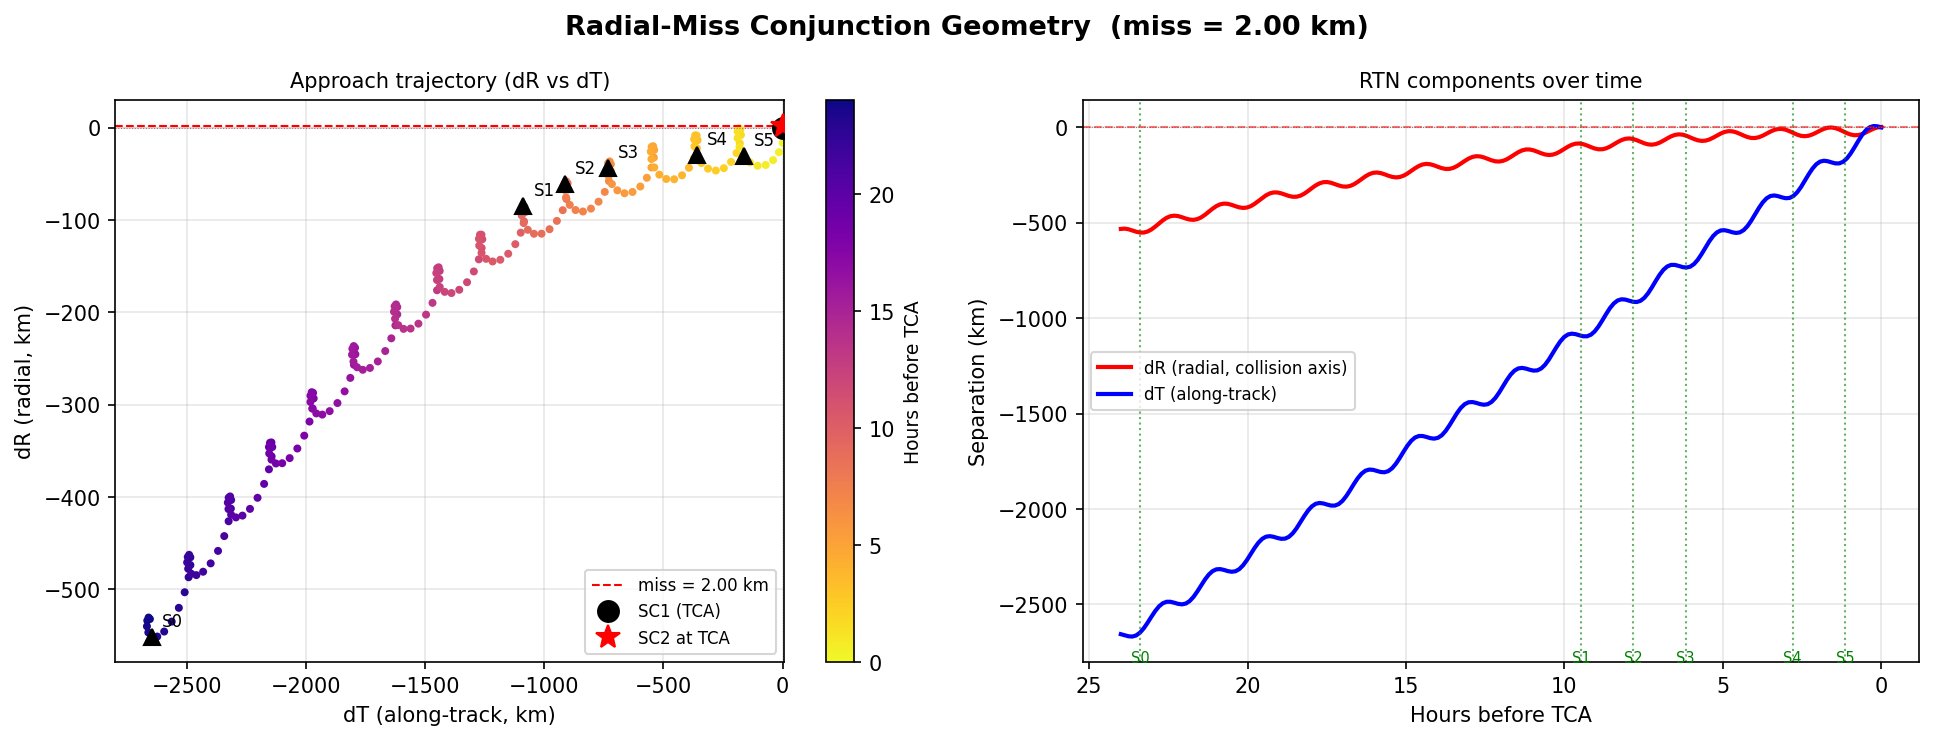
\includegraphics[width=\linewidth]{../figures/conjunction_geometry.png}
      \vspace{0.3em}
      \small $\Delta v_T$ (along-track burn) shifts $d_\text{miss}$ predictably\\
      Along-track burns differentiate bins at all planning stages
    \end{column}
  \end{columns}
  \vspace{0.3em}
  \begin{alertblock}{Why not crossing geometry?}
    Crossing = miss in N (cross-track). N collapses to a single bin --- collision zone
    is unreachable from nominal RTN trajectories. Radial-miss puts the collision
    axis directly in state.
  \end{alertblock}
\end{frame}

\begin{frame}{Transition Model}
  \begin{block}{Built offline with Brahe --- RS-SDA* never calls Brahe}
  \end{block}
  \vspace{0.5em}
  For each $(d_\text{miss\_bin},\; k,\; a)$:
  \begin{enumerate}
    \item \textbf{Place SC2 at TCA} with target miss distance in RTN,
          then back-propagate to stage epoch $\tau_k$
    \item Apply joint maneuver $(a_1, a_2)$ impulsively to SC1 and SC2
    \item \textbf{Brahe-propagate} both spacecraft from $\tau_k$ to TCA
    \item Measure resulting miss distance $d'$ $\rightarrow$ bin it $\rightarrow$ next state
  \end{enumerate}
  \vspace{0.3em}
  \begin{block}{Why back-propagation?}
    Placing SC2 at a radial offset \emph{at the stage epoch} produces the wrong miss
    at TCA --- the offset evolves under Keplerian dynamics, diverging by thousands of km
    over 24\,h. Back-propagating from TCA guarantees the representative trajectory
    has exactly the target miss distance ($< 1$\,m error across all bins and stages).
  \end{block}
  \vspace{0.2em}
  \begin{alertblock}{Key property}
    Collision reward fires correctly because miss distance IS the state.
  \end{alertblock}
\end{frame}

\begin{frame}{Reward Function}
  \[
    R(s, a) = R_\text{collision}(s) + R_\text{maneuver}(a) + R_\text{comms}(a)
  \]
  \vspace{0.5em}
  \begin{itemize}
    \item \textbf{Collision penalty} (terminal):
      \[
        R_\text{collision} = \begin{cases} -1000 & d_\text{miss} < 1\,\text{km} \\ 0 & \text{otherwise} \end{cases}
      \]
    \item \textbf{Maneuver cost} (fuel / trajectory deviation proxy):
      \[
        R_\text{maneuver} = -10 \cdot \mathbf{1}[a_1 \neq \text{WAIT}]
                            -10 \cdot \mathbf{1}[a_2 \neq \text{WAIT}]
      \]
    \item \textbf{Communication cost} (Scenario 3):
      \[
        R_\text{comms} = -c_\text{sync} \cdot \mathbf{1}[\text{sync at this stage}]
      \]
  \end{itemize}
  \vspace{0.3em}
  \TODO{Add trajectory deviation: penalize change in orbital elements accumulated over all maneuvers}
\end{frame}

% =============================================================================
\section{Communication Structure}
% =============================================================================

\begin{frame}{Synchronization Triggers}
  Ground-station contacts define \textbf{when agents can share beliefs and coordinate}\\[0.3em]
  \small\textit{Contact windows computed with Brahe from real GS geometry (Goddard, 550\,km LEO, 55° incl.)}

  \vspace{0.5em}
  \begin{center}
  \begin{tabular}{lccc}
    \toprule
    Stage & Time before TCA & Scenario 1 & Scenario 2 \\
    \midrule
    0 & $T{-}23.4$\,h & \good{Joint} & \good{Joint} \\
    1 & $T{-}9.5$\,h  & \good{Joint} & \good{Joint} \\
    2 & $T{-}7.8$\,h  & \good{Joint} & \good{Joint} \\
    3 & $T{-}6.2$\,h  & \good{Joint} & \bad{SC1 only} \\
    4 & $T{-}2.8$\,h  & \good{Joint} & \bad{SC1 only} \\
    5 & $T{-}1.1$\,h  & \good{Joint} & \bad{SC1 only} \\
    \bottomrule
  \end{tabular}
  \end{center}
  \vspace{0.3em}
  Scenario 1: both SC in similar orbits $\Rightarrow$ all 6 passes are simultaneous $\Rightarrow$ always joint\\
  Scenario 3: all stages available but sync costs $c_\text{sync}$ per event
\end{frame}

% =============================================================================
\section{Three Scenarios}
% =============================================================================

\begin{frame}{Scenario 1: Cooperative Shared Operator}
  \begin{itemize}
    \item Both SC controlled by one operator, single ground station (Goddard)
    \item All 6 contacts are joint sync triggers $\rightarrow$ always centralized
  \end{itemize}
  \vspace{0.5em}
  \begin{block}{Experiment}
    Vary ground network density:
    \begin{itemize}
      \item \textbf{Dense} (6--12 stations globally): many syncs, near-centralized
      \item \textbf{Regional} (1--3 stations): fewer syncs, more decentralized
    \end{itemize}
  \end{block}
  \vspace{0.5em}
  \textbf{Baselines}: centralized (perfect info), decentralized (no sync), SDec (ours)\\[0.3em]
  \textbf{Expected result}: $V_\text{dec} \leq V_\text{sdec} \leq V_\text{cen}$, with $V_\text{sdec} \approx V_\text{cen}$ using few syncs
\end{frame}

\begin{frame}{Scenario 2: Asymmetric Control}
  \begin{itemize}
    \item SC1: fully controllable (our agent)
    \item SC2: follows a \textbf{fixed third-party policy} (unknown to SC1)
  \end{itemize}
  \vspace{0.5em}
  \begin{columns}
    \begin{column}{0.48\textwidth}
      \begin{block}{SC2 policy variants}
        \begin{itemize}
          \item \textit{Uncooperative}: never maneuvers
          \item \textit{Reactive}: maneuvers if predicted miss $< \theta$ at its contact, $\theta$ unknown to SC1
        \end{itemize}
      \end{block}
    \end{column}
    \begin{column}{0.48\textwidth}
      SC1 plans \textbf{conservatively} under uncertainty about SC2's behavior and maneuver timing
      \vspace{0.5em}

      \TODO{Define how SC2's fixed policy is encoded in transition matrix}
    \end{column}
  \end{columns}
\end{frame}

\begin{frame}{Scenario 3: Costly Communication}
  \begin{itemize}
    \item Same contact structure as Scenario 1
    \item Each sync event incurs penalty $c_\text{sync}$ in reward
  \end{itemize}
  \vspace{0.5em}
  \begin{block}{Trade-off}
    \begin{itemize}
      \item \good{Sync} $\rightarrow$ better joint belief, coordinated action, safer
      \item \bad{Sync} $\rightarrow$ costs $c_\text{sync}$ per event
    \end{itemize}
  \end{block}
  \vspace{0.5em}
  \textbf{Experiment}: sweep $c_\text{sync}$ from 0 to 100\\[0.3em]
  \textbf{Measure}: optimal sync count and resulting miss distance\\[0.3em]
  \textbf{Key question}: what is the minimum communication required for safe CA?
\end{frame}

% =============================================================================
\section{System Architecture}
% =============================================================================

\begin{frame}{System Architecture}
  \begin{columns}
    \begin{column}{0.48\textwidth}
      \textbf{Three separate components:}
      \vspace{0.5em}
      \begin{enumerate}
        \item \textbf{Matrix Builder} (offline, once)\\
              \texttt{spacecraft\_matrices.py}\\
              Brahe $\rightarrow$ T, O, R $\rightarrow$ .npz
        \vspace{0.5em}
        \item \textbf{Policy Solver} (offline)\\
              \texttt{sdec\_spacecraft.py}\\
              .npz $\rightarrow$ RS-SDA* $\rightarrow$ policy
        \vspace{0.5em}
        \item \textbf{Simulator} (evaluation)\\
              \texttt{spacecraft\_simulator.py}\\
              Policy + Brahe $\rightarrow$ metrics
      \end{enumerate}
    \end{column}
    \begin{column}{0.48\textwidth}
      \begin{block}{Key separation}
        RS-SDA* \textbf{never calls Brahe}.\\
        Brahe runs offline to build matrices, then again in the simulator to evaluate the policy with real ECI states.
      \end{block}
      \vspace{0.5em}
      \begin{alertblock}{Simulator metrics}
        \begin{itemize}
          \item Minimum miss distance at TCA
          \item Total $\Delta v$ accumulated
          \item Sync event count \& timing
          \item \TODO{Trajectory deviation}
        \end{itemize}
      \end{alertblock}
    \end{column}
  \end{columns}
\end{frame}

% =============================================================================
\section{Status \& Next Steps}
% =============================================================================

\begin{frame}{Implementation Status}
  \begin{columns}
    \begin{column}{0.48\textwidth}
      \textbf{Infrastructure} \good{(all done)}
      \begin{itemize}\small
        \item GS contact windows (\texttt{test\_contacts.py})
        \item Conjunction geometry (\texttt{test\_conjunction\_geometry.py})
        \item Miss-distance discretizer
        \item Matrix builder (T, O, R via Brahe)
        \item Policy solver (RS-SDA* wrapper)
        \item Simulator (RS-SDA* + greedy rollout)
      \end{itemize}
    \end{column}
    \begin{column}{0.48\textwidth}
      \textbf{Experiments \& tuning} \good{(all done)}
      \begin{itemize}\small
        \item Scenario 1 comparison (100 rollouts, 3 variants)
        \item Scenario 3 costly-comms sweep ($c \in [0,200]$)
        \item Bin-1 terminal penalty ($R=-200$)
        \item Obs noise tuned to $\sigma=5$\,km
        \item Policy grid visualization
      \end{itemize}
      \vspace{0.5em}
      \textbf{Pending}
      \begin{itemize}\small
        \item Scenario 3 structural fix (optional sync)
        \item Scenario 2 (asymmetric control)
        \item Reward shaping, finer bins
      \end{itemize}
    \end{column}
  \end{columns}
\end{frame}

\begin{frame}{Scenario 1 Results (after bin-1 fix)}
  \begin{block}{100 rollouts, dv = 0.5\,m/s, $\sigma_\text{obs}=5$\,km, bin-1 penalty $=-200$}
  \end{block}
  \vspace{0.4em}
  \begin{center}
  \begin{tabular}{lccrrr}
    \toprule
    Policy & Init bin & Coll.\% & Mean miss & Mean dv & Syncs \\
    \midrule
    Centralized   & 0 & \good{0.0} & 127.8\,km & 0.50\,m/s & 6.0 \\
    Decentralized & 0 & \good{0.0} & 128.0\,km & 0.50\,m/s & 0.0 \\
    SDec          & 0 & \good{0.0} & 127.8\,km & 0.50\,m/s & 6.0 \\
    \midrule
    Centralized   & 1 & \good{0.0} & 127.9\,km & 0.50\,m/s & 6.0 \\
    Decentralized & 1 & \good{0.0} & 128.1\,km & 0.50\,m/s & 0.0 \\
    SDec          & 1 & \good{0.0} & 127.9\,km & 0.50\,m/s & 6.0 \\
    \bottomrule
  \end{tabular}
  \end{center}
  \vspace{0.4em}
  \begin{alertblock}{Current limitation}
    One decisive early burn = all three variants near-identical ($<0.3$\,km difference).
    Observation asymmetry is now physically correct but policy timing is unchanged.
    Next: trajectory deviation state to penalize early burns and force timing tradeoffs.
  \end{alertblock}
\end{frame}

\begin{frame}{Scenario 3: Structural Issue Found}
  \begin{alertblock}{Sync count fixed at 6 regardless of $c_\text{sync}$}
    Policy value degrades linearly ($-10, -130, \ldots, -1210$) but sync count stays at 6.
    Root cause: all states are \texttt{sync\_states} $\Rightarrow$ sync is mandatory, not optional.
  \end{alertblock}
  \vspace{0.5em}
  \textbf{Fix required}: model sync as a \emph{choice} during contact windows via
  \texttt{sync\_actions} or \texttt{sync\_observations} in RSSDA, so the policy can
  trade off communication cost against collision risk.

\end{frame}

\begin{frame}{Next Steps}
  \begin{enumerate}
    \item \textbf{Deviation-from-nominal state} --- expand state to
          $(d_\text{miss},\; \delta_1,\; \delta_2,\; k)$ where $\delta_i$ bins
          SC$i$'s along-track displacement from its no-burn trajectory at TCA\\
          \small 4 bins per SC: $[0,2)$, $[2,20)$, $[20,60)$, $[60+)$\,km $\rightarrow$ 577 states total\\
          Reward penalty $-\alpha(\delta_1 + \delta_2)$ per stage discourages early burns
    \vspace{0.2em}
    \item \textbf{Intermediate non-contact timesteps} --- add 1--2 decentralized-only
          steps in the 14\,h gap (stages 0$\rightarrow$1) to force richer sequential decisions
    \vspace{0.2em}
    \item \textbf{Scenario 3 fix}: make sync optional via \texttt{sync\_actions} ---
          encode ``communicate'' vs.\ ``don't communicate'' as a deliberate choice
    \vspace{0.2em}
    \item \textbf{Scenario 2}: SC2 uncooperative ---
          $T_\text{asym}[a,s,s'] = T_\text{full}[a_1 \cdot 3,\, s,\, s']$
    \vspace{0.2em}
    \item \textbf{Obs noise sweep}: compare variants at $\sigma \in \{1, 5, 20\}$\,km
    \vspace{0.2em}
    \item \textbf{J2 perturbations}: upgrade from two-body to J2 propagator in Brahe
  \end{enumerate}
\end{frame}

\begin{frame}{Script Run Order}
  \small Run all from repo root: \texttt{.venv/bin/python spacecraftCA/<script>.py}
  \vspace{0.3em}
  \begin{center}
  \begin{tabular}{lll}
    \toprule
    Step & Script & Notes \\
    \midrule
    1 & \texttt{spacecraft\_matrices.py --force} & Build T,O,R ($\sim$2\,min) \\
    2 & \texttt{spacecraft\_discretizer.py} & Verify matrices \\
    3 & \texttt{sdec\_spacecraft.py} & Solve, print value \\
    4 & \texttt{spacecraft\_simulator.py --compare} & Sc.\ 1 comparison \\
    5 & \texttt{scenario3\_sweep.py --c-max 200} & Sc.\ 3 sweep \\
    6 & \texttt{plot\_policy.py} & Policy grid ($\sim$10\,min) \\
    7 & \texttt{plot\_conjunction\_geometry.py} & RTN plot / GIF \\
    \bottomrule
  \end{tabular}
  \end{center}
  \vspace{0.3em}
  Recompile docs from \texttt{notes/report/} and \texttt{notes/slides/}:\\
  \texttt{pdflatex formulation.tex} \quad / \quad \texttt{pdflatex slides.tex}
\end{frame}

\begin{frame}{Summary}
  \begin{itemize}
    \item Modeled spacecraft CA as SDec-POMDP with ground contacts as sync triggers
    \vspace{0.5em}
    \item \textbf{State}: predicted miss distance at TCA --- clean connection to reward,
          matches CDM reporting
    \vspace{0.5em}
    \item \textbf{Dynamics}: Brahe offline for T matrix; RS-SDA* operates on arrays only
    \vspace{0.5em}
    \item \textbf{Three scenarios} quantify how contact frequency, symmetry,
          and cost shape safety vs.\ communication overhead
    \vspace{0.5em}
    \item \textbf{Expected result}: planned synchronizations achieve near-centralized
          safety with fewer communications
  \end{itemize}
\end{frame}

\end{document}
